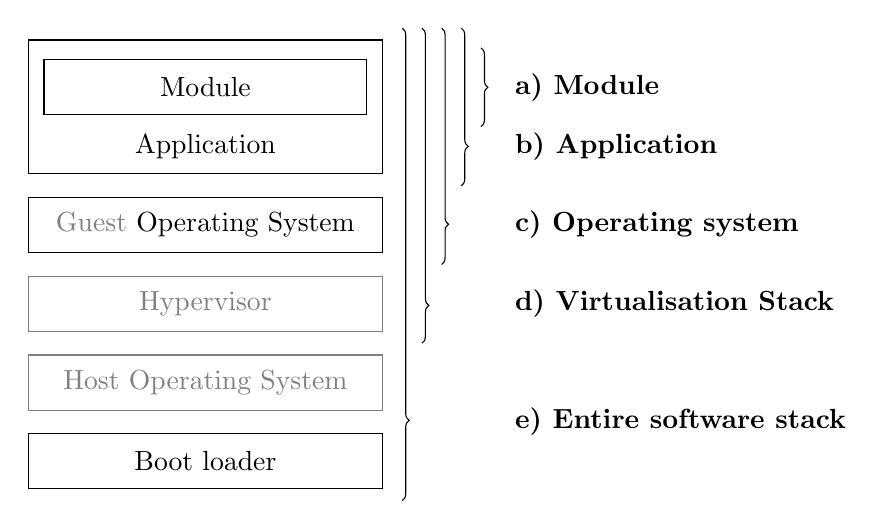
\begin{tikzpicture}[
  nodes={draw, text width=4.5cm, inner sep=0, minimum height=0.7cm, align=center},
  optional/.style={color=gray, draw=gray},
  label/.style={draw=none, align=left, inner sep=5pt, font=\bfseries, text width={}, align=left}
]

\node (bl) at (-0.5,-1.5) {Boot loader};
\node [optional] (os1) at (-0.5,-0.5) {Host Operating System};
\node [optional] (hyp) at (-0.5,0.5) {Hypervisor};
\node (os2) at (-0.5,1.5) {\textcolor{gray}{Guest} Operating System};
\node [draw=none] (app) at (-0.5,2.5) {Application};
\node [text width=4.1cm] (mod) at (-0.5,3.25) {Module};
\draw (-2.75,3.85) rectangle (1.75,2.15);

\node [label, right] at (3.25,3.25) {a) Module};
\draw[decorate, decoration={brace, mirror}] (3,2.75) -- (3,3.75);

\node [label, right] at (3.25,2.5) {b) Application};
\draw[decorate, decoration={brace, mirror, aspect=0.25}] (2.75,2) -- (2.75,4);

\node [label, right] at (3.25,1.5) {c) Operating system};
\draw[decorate, decoration={brace, mirror, aspect=0.17}] (2.5,1) -- (2.5,4);

\node [label, right] at (3.25,0.5) {d) Virtualisation Stack};
\draw[decorate, decoration={brace, mirror, aspect=0.12}] (2.25,0) -- (2.25,4);

\node [label, right] at (3.25,-1) {e) Entire software stack};
\draw[decorate, decoration={brace, mirror, aspect=0.17}] (2,-2) -- (2,4);

\end{tikzpicture}
